\documentclass[12pt,letterpaper]{article}
\usepackage[utf8]{inputenc}
\usepackage[T1]{fontenc}
\usepackage{lmodern}
\usepackage{graphicx}
\usepackage{caption}
\captionsetup{
    font=small,
    labelfont=bf,
    textfont=md,
    format=hang,
    justification=centering,
    textformat=period,
}
\usepackage{float}
\usepackage{geometry}
\usepackage{microtype}
\usepackage[breaklinks=true,hidelinks]{hyperref}
\usepackage{listings}
\usepackage{xcolor}
\usepackage[most]{tcolorbox}
\usepackage{amsmath}
\usepackage{cleveref}
\usepackage{textcomp}
 \newcommand{\mytexttilde}{\raisebox{0.5ex}{\texttildelow}}
% Set page margins
% \geometry{
%     a4paper,
%     left=25mm,
%     right=25mm,
%     top=25mm,
%     bottom=25mm,
% }

% Define custom style for listings
\lstdefinestyle{custombash}{
    language=bash,
    basicstyle=\ttfamily\small,
    keywordstyle=\color{blue},
    commentstyle=\color{gray},
    stringstyle=\color{red},
    backgroundcolor=\color{gray!10},
    frame=single,
    breaklines=true,
    showstringspaces=false,
}

\begin{document}

\title{\LARGE IQmol Setup Guide}
\author{Markus G. S. Weiss}
\date{2024/10/28}
\maketitle

\tableofcontents
\newpage
\section{Introduction}

This guide will walk you through configuring IQmol to connect to the cluster and submit jobs. If you plan to use SSH key authentication, ensure that you have already generated SSH keys and uploaded your public key to the server. If you prefer to use password authentication, you can proceed without setting up SSH keys.

\section{Configuring IQmol}

Follow the steps below to set up the server details in IQmol.

\subsection*{Setting Up the Server Details}

\begin{enumerate}
    \item Open IQmol.
    \item Navigate to \textbf{Calculation} $\rightarrow$ \textbf{Edit Servers}.

    \begin{figure}[H]
        \centering
        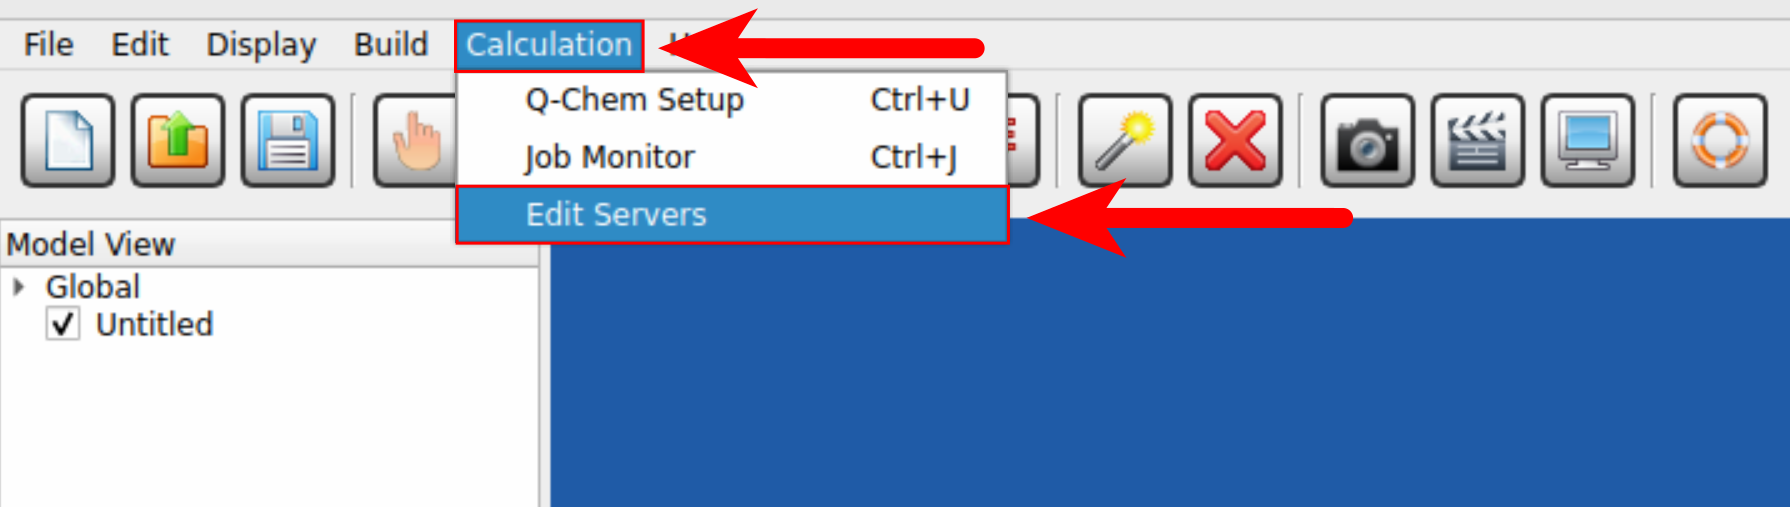
\includegraphics[width=0.8\textwidth]{iqmol_edit_servers.png}
        \caption{Accessing Edit Servers in IQmol}
        \label{fig:iqmol_edit_servers}
    \end{figure}

    \item Click on the \textbf{+} button to create a new server configuration.

    \begin{figure}[H]
        \centering
        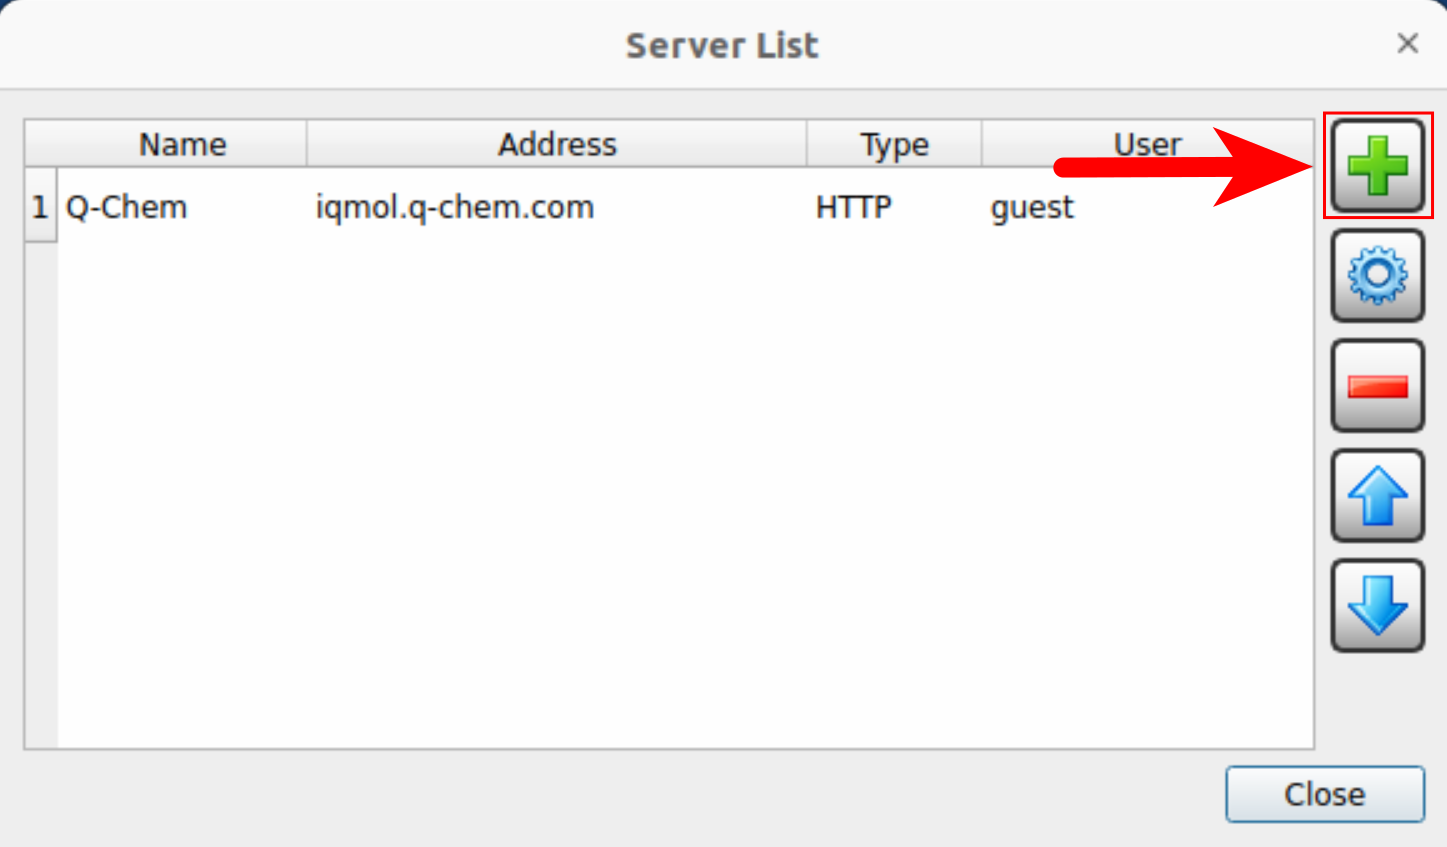
\includegraphics[width=0.8\textwidth]{iqmol_add_server.png}
        \caption{Add New Server in IQmol}
        \label{fig:iqmol_add_server}
    \end{figure}

    The server configuration window will appear with numbered fields as shown below. Follow the instructions corresponding to each number:

    \begin{figure}[H]
        \centering
        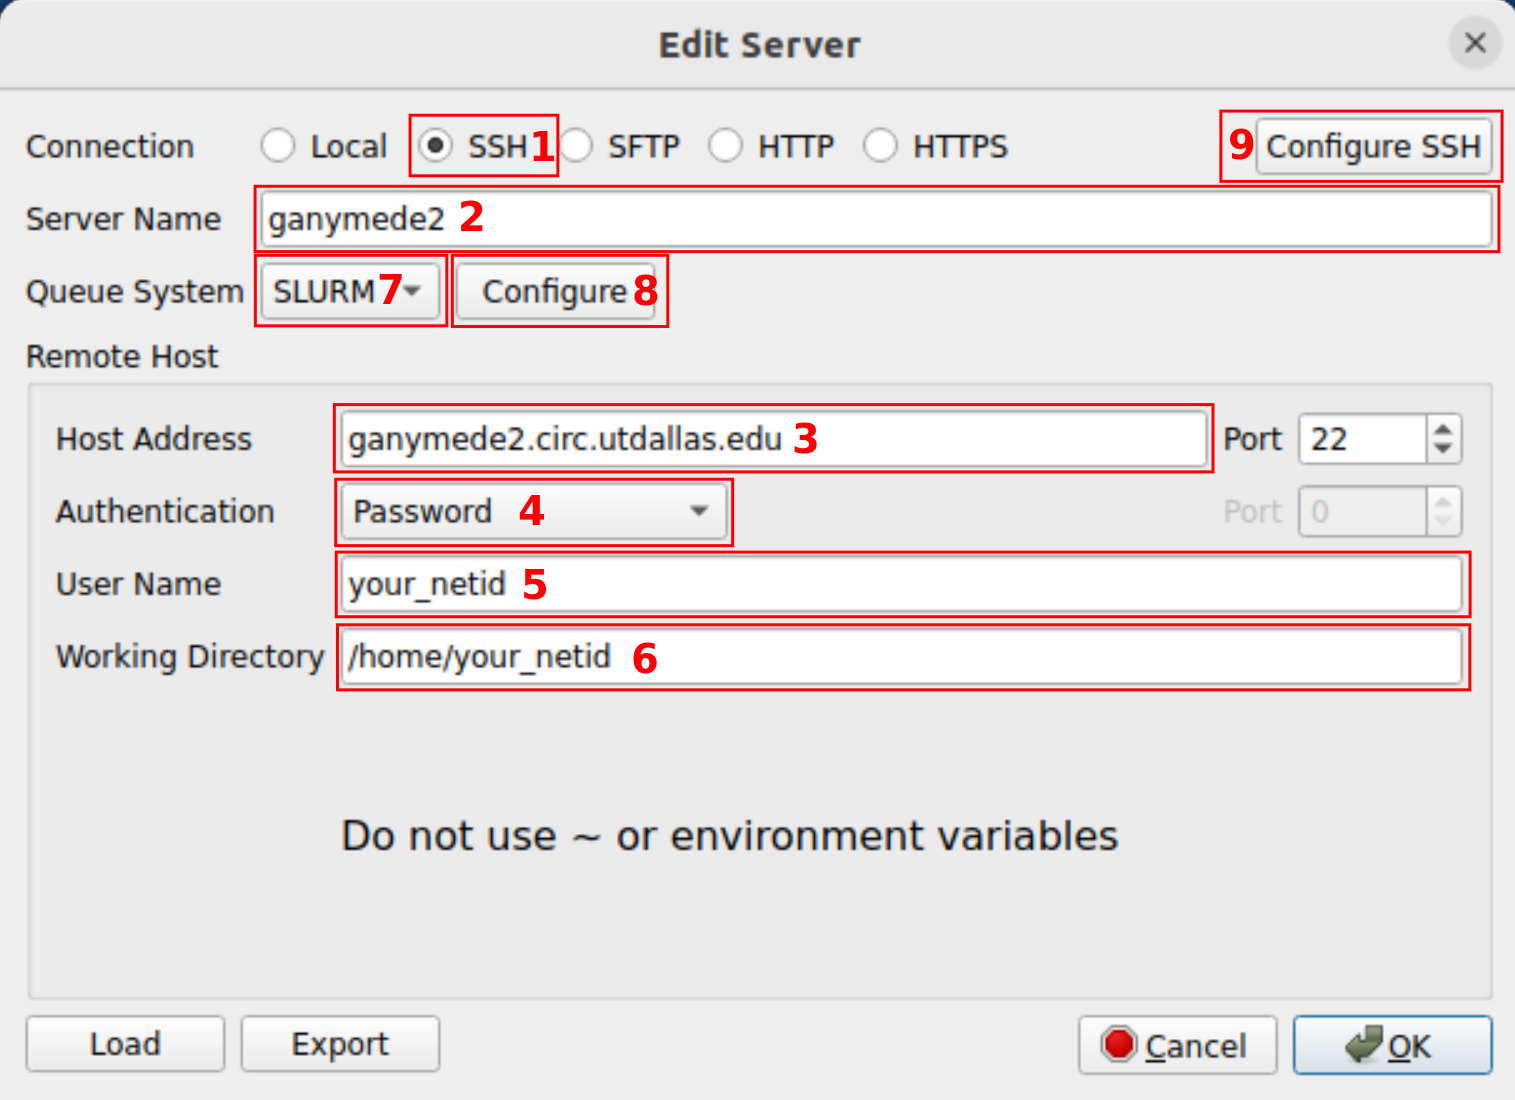
\includegraphics[width=0.8\textwidth]{iqmol_server_configuration_numbered.png}
        \caption{Server Configuration Window}
        \label{fig:iqmol_server_configuration}
    \end{figure}

    \begin{enumerate}
        \item[\textbf{1.}] \textbf{Connection}: Select \textbf{SSH} as the connection method.
        \item[\textbf{2.}] \textbf{Name}: Enter a recognizable server name, such as \texttt{ganymede2}.
        \item[\textbf{3.}] \textbf{Host Address}: Enter
        \begin{lstlisting}[style=custombash]
ganymede2.circ.utdallas.edu
        \end{lstlisting}
        \item[\textbf{4.}] \textbf{Authentication}: Choose the appropriate method:
        \begin{itemize}
            \item If you set up SSH keys, select \textbf{Public Key}.
            \item If using an SSH agent, select \textbf{Agent}.
            \item If you prefer to use a password, select \textbf{Password}.
        \end{itemize}
        \item[\textbf{5.}] \textbf{Username}: Enter your \textbf{NetID}.
        \item[\textbf{6.}] \textbf{Working Directory}: Set to \texttt{/home/your\_netid}, replacing \texttt{your\_netid} with your actual NetID.
        \item[\textbf{7.}] \textbf{Queue System}: Select \textbf{Slurm} from the dropdown menu.
        \item[\textbf{8.}] \textbf{Configure Queue System}:
        \begin{enumerate}
            \item Click on \textbf{Configure Queue System}. A new window will appear.

            \begin{figure}[H]
                \centering
                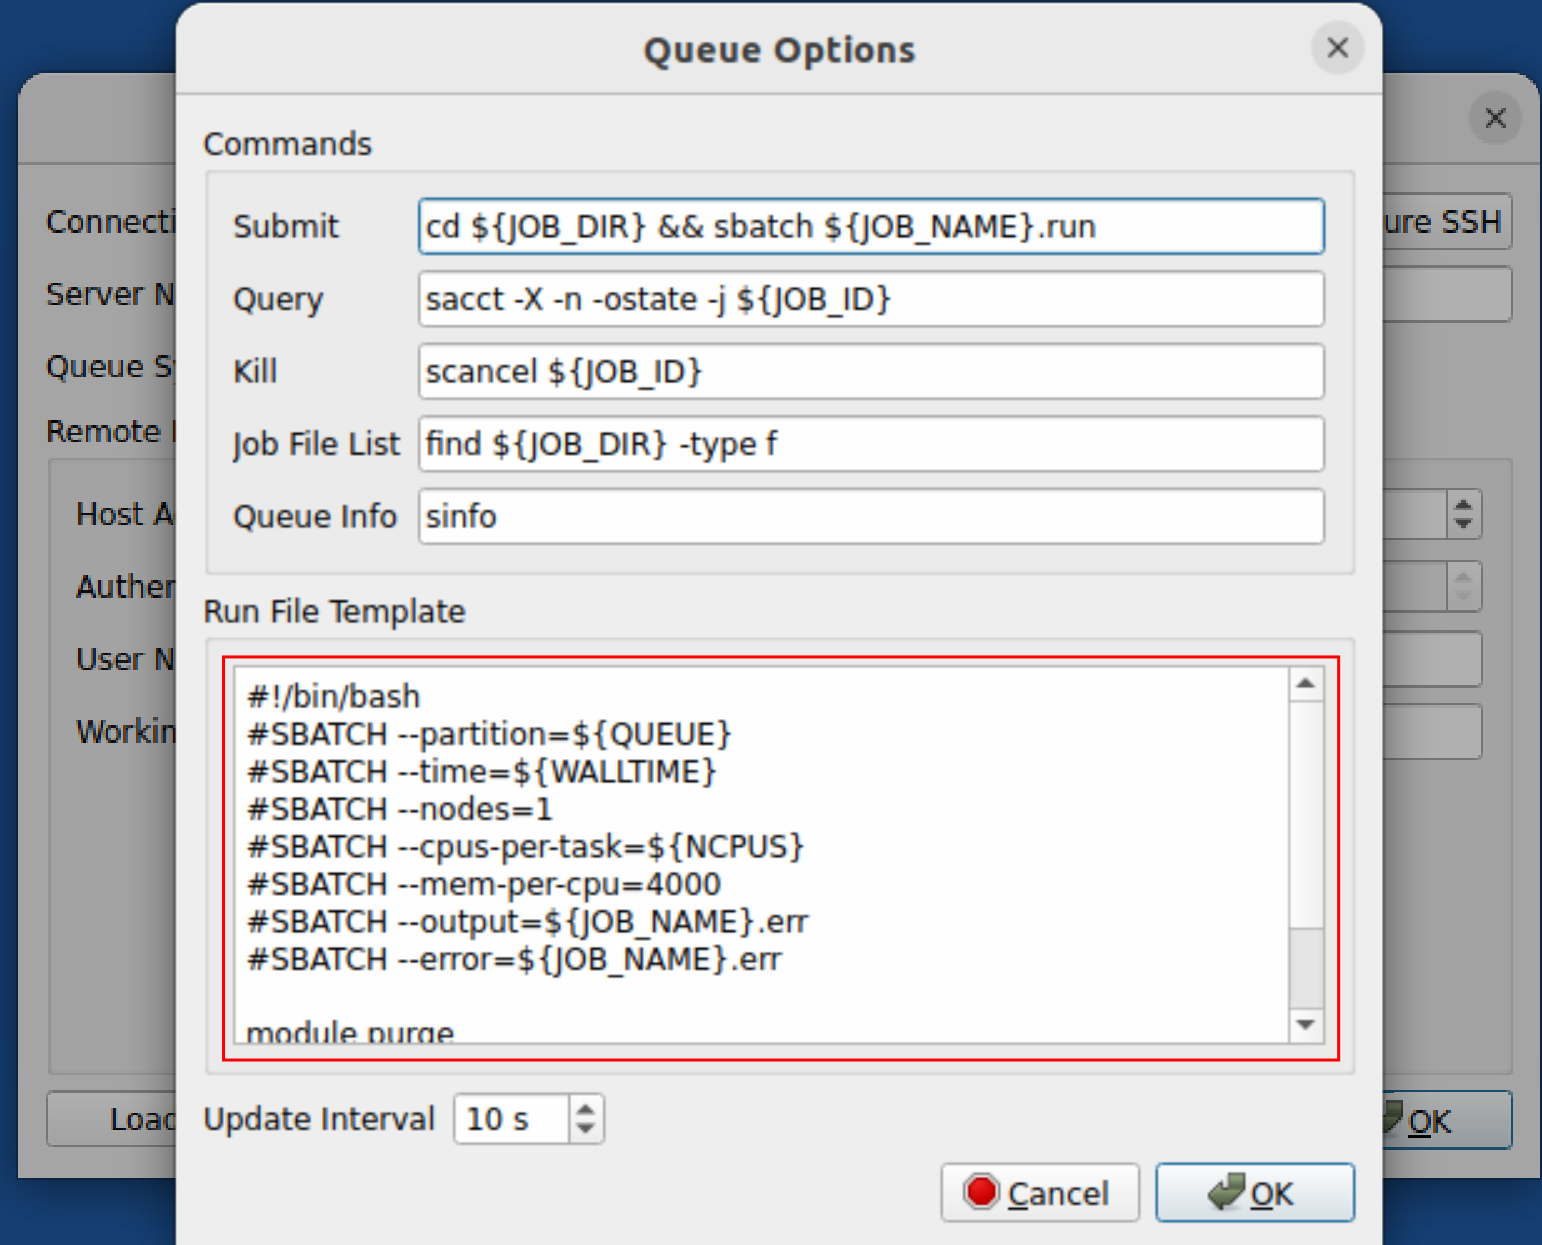
\includegraphics[width=0.8\textwidth]{iqmol_queue_system_configuration.png}
                \caption{Queue System Configuration}
                \label{fig:iqmol_queue_system_configuration}
            \end{figure}

            \item In the \textbf{Setup Commands} section, delete any existing lines and add the following lines:

            \begin{lstlisting}[style=custombash]
#!/bin/bash
#SBATCH --partition=${QUEUE}
#SBATCH --time=${WALLTIME}
#SBATCH --nodes=1
#SBATCH --cpus-per-task=${NCPUS}
#SBATCH --mem-per-cpu=4000
#SBATCH --output=${JOB_NAME}.err
#SBATCH --error=${JOB_NAME}.err

module purge
module load qchem/6.2.1

qchem -nt ${NCPUS} ${JOB_NAME}.inp ${JOB_NAME}.out
            \end{lstlisting}

            \item Click \textbf{OK} to save the queue system configuration.
        \end{enumerate}
        \item[\textbf{9.}] \textbf{Configure SSH}:
        \begin{enumerate}
            \item Click on \textbf{Configure SSH}. A new window will appear.

            \item For the \textbf{Known Hosts File}:
            \begin{itemize}
                \item Ensure that the \texttt{\mytexttilde/.ssh} directory exists.
                \item For \textbf{Windows Users}:
                \begin{itemize}
                    \item If the directory does not exist, create it at \texttt{\%USERPROFILE\%\textbackslash.ssh}.
                \end{itemize}
                \item For \textbf{macOS/Linux Users}:
                \begin{itemize}
                    \item The directory should exist at \texttt{\mytexttilde/.ssh}.
                \end{itemize}
            \end{itemize}

            \item The \textbf{Known Hosts File} path:

            \begin{itemize}
                \item For Linux:
                \begin{lstlisting}[style=custombash]
/home/your_local_username/.ssh/known_hosts
                \end{lstlisting}
                \item For macOS:
                \begin{lstlisting}[style=custombash]
/Users/your_local_username/.ssh/known_hosts
                \end{lstlisting}
                \item For Windows:
                \begin{lstlisting}[style=custombash]
C:\Users\your_local_username\.ssh\known_hosts
                \end{lstlisting}
            \end{itemize}

            \item If you selected \textbf{Password} authentication:
            \begin{itemize}
                \item You can leave the \textbf{Private Key File} and \textbf{Public Key File} fields empty.
            \end{itemize}

            \item If you selected \textbf{Public Key} authentication:
            \begin{itemize}
                \item Set the \textbf{Private Key File} to your private key, e.g.,\\
                For Linux:
                \begin{lstlisting}[style=custombash]
/home/your_local_username/.ssh/id_ed25519
                \end{lstlisting}
                For macOS:
                \begin{lstlisting}[style=custombash]
/Users/your_local_username/.ssh/id_ed25519
                \end{lstlisting}
                For Windows:
                \begin{lstlisting}[style=custombash]
C:\Users\your_local_username\.ssh\id_ed25519
                \end{lstlisting}
                \item Set the \textbf{Public Key File} to your public key, e.g.,\\
                For Linux:
                \begin{lstlisting}[style=custombash]
/home/your_local_username/.ssh/id_ed25519.pub
                \end{lstlisting}
                For macOS:
                \begin{lstlisting}[style=custombash]
/Users/your_local_username/.ssh/id_ed25519.pub
                \end{lstlisting}
                For Windows:
                \begin{lstlisting}[style=custombash]
C:\Users\your_local_username\.ssh\id_ed25519.pub
                \end{lstlisting}
            \end{itemize}

            \item If you selected \textbf{Agent} authentication:
            \begin{itemize}
                \item Ensure your SSH agent is running and has your key added.
                \item Leave the \textbf{Private Key File} and \textbf{Public Key File} fields empty.
            \end{itemize}

            \item Click \textbf{OK} to save the SSH configuration.

            \begin{figure}[H]
                \centering
                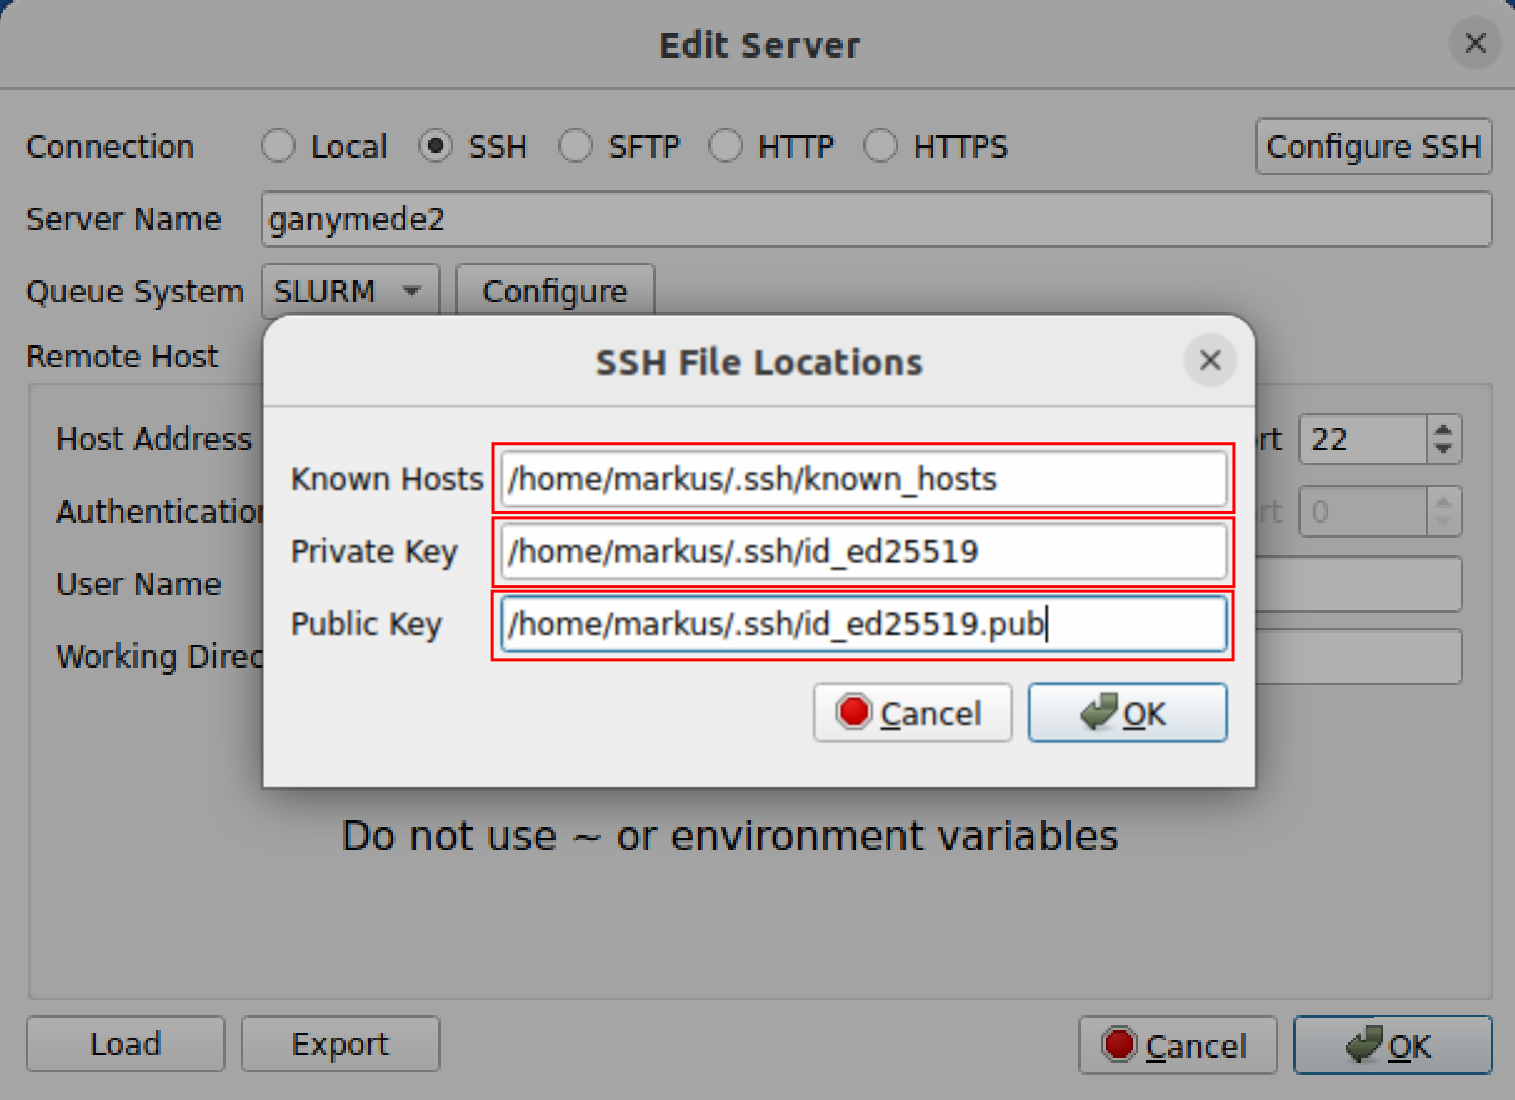
\includegraphics[width=0.8\textwidth]{iqmol_ssh_configuration.png}
                \caption{SSH Configuration}
                \label{fig:iqmol_ssh_configuration}
            \end{figure}
        \end{enumerate}
    \end{enumerate}

    \item Click \textbf{OK} to save the server settings. You may use the arrow keys in \cref{fig:iqmol_add_server} to move your created server up as the default.
\end{enumerate}
\newpage
\section{Submitting a Job in IQmol}

\begin{enumerate}
    \item Prepare your calculation in IQmol as usual.
    \item When ready to submit, navigate to \textbf{Calculation} $\rightarrow$ \textbf{Q-Chem Setup}.
    \item Select your created server (\texttt{ganymede2}) from the list.

    \begin{figure}[H]
        \centering
        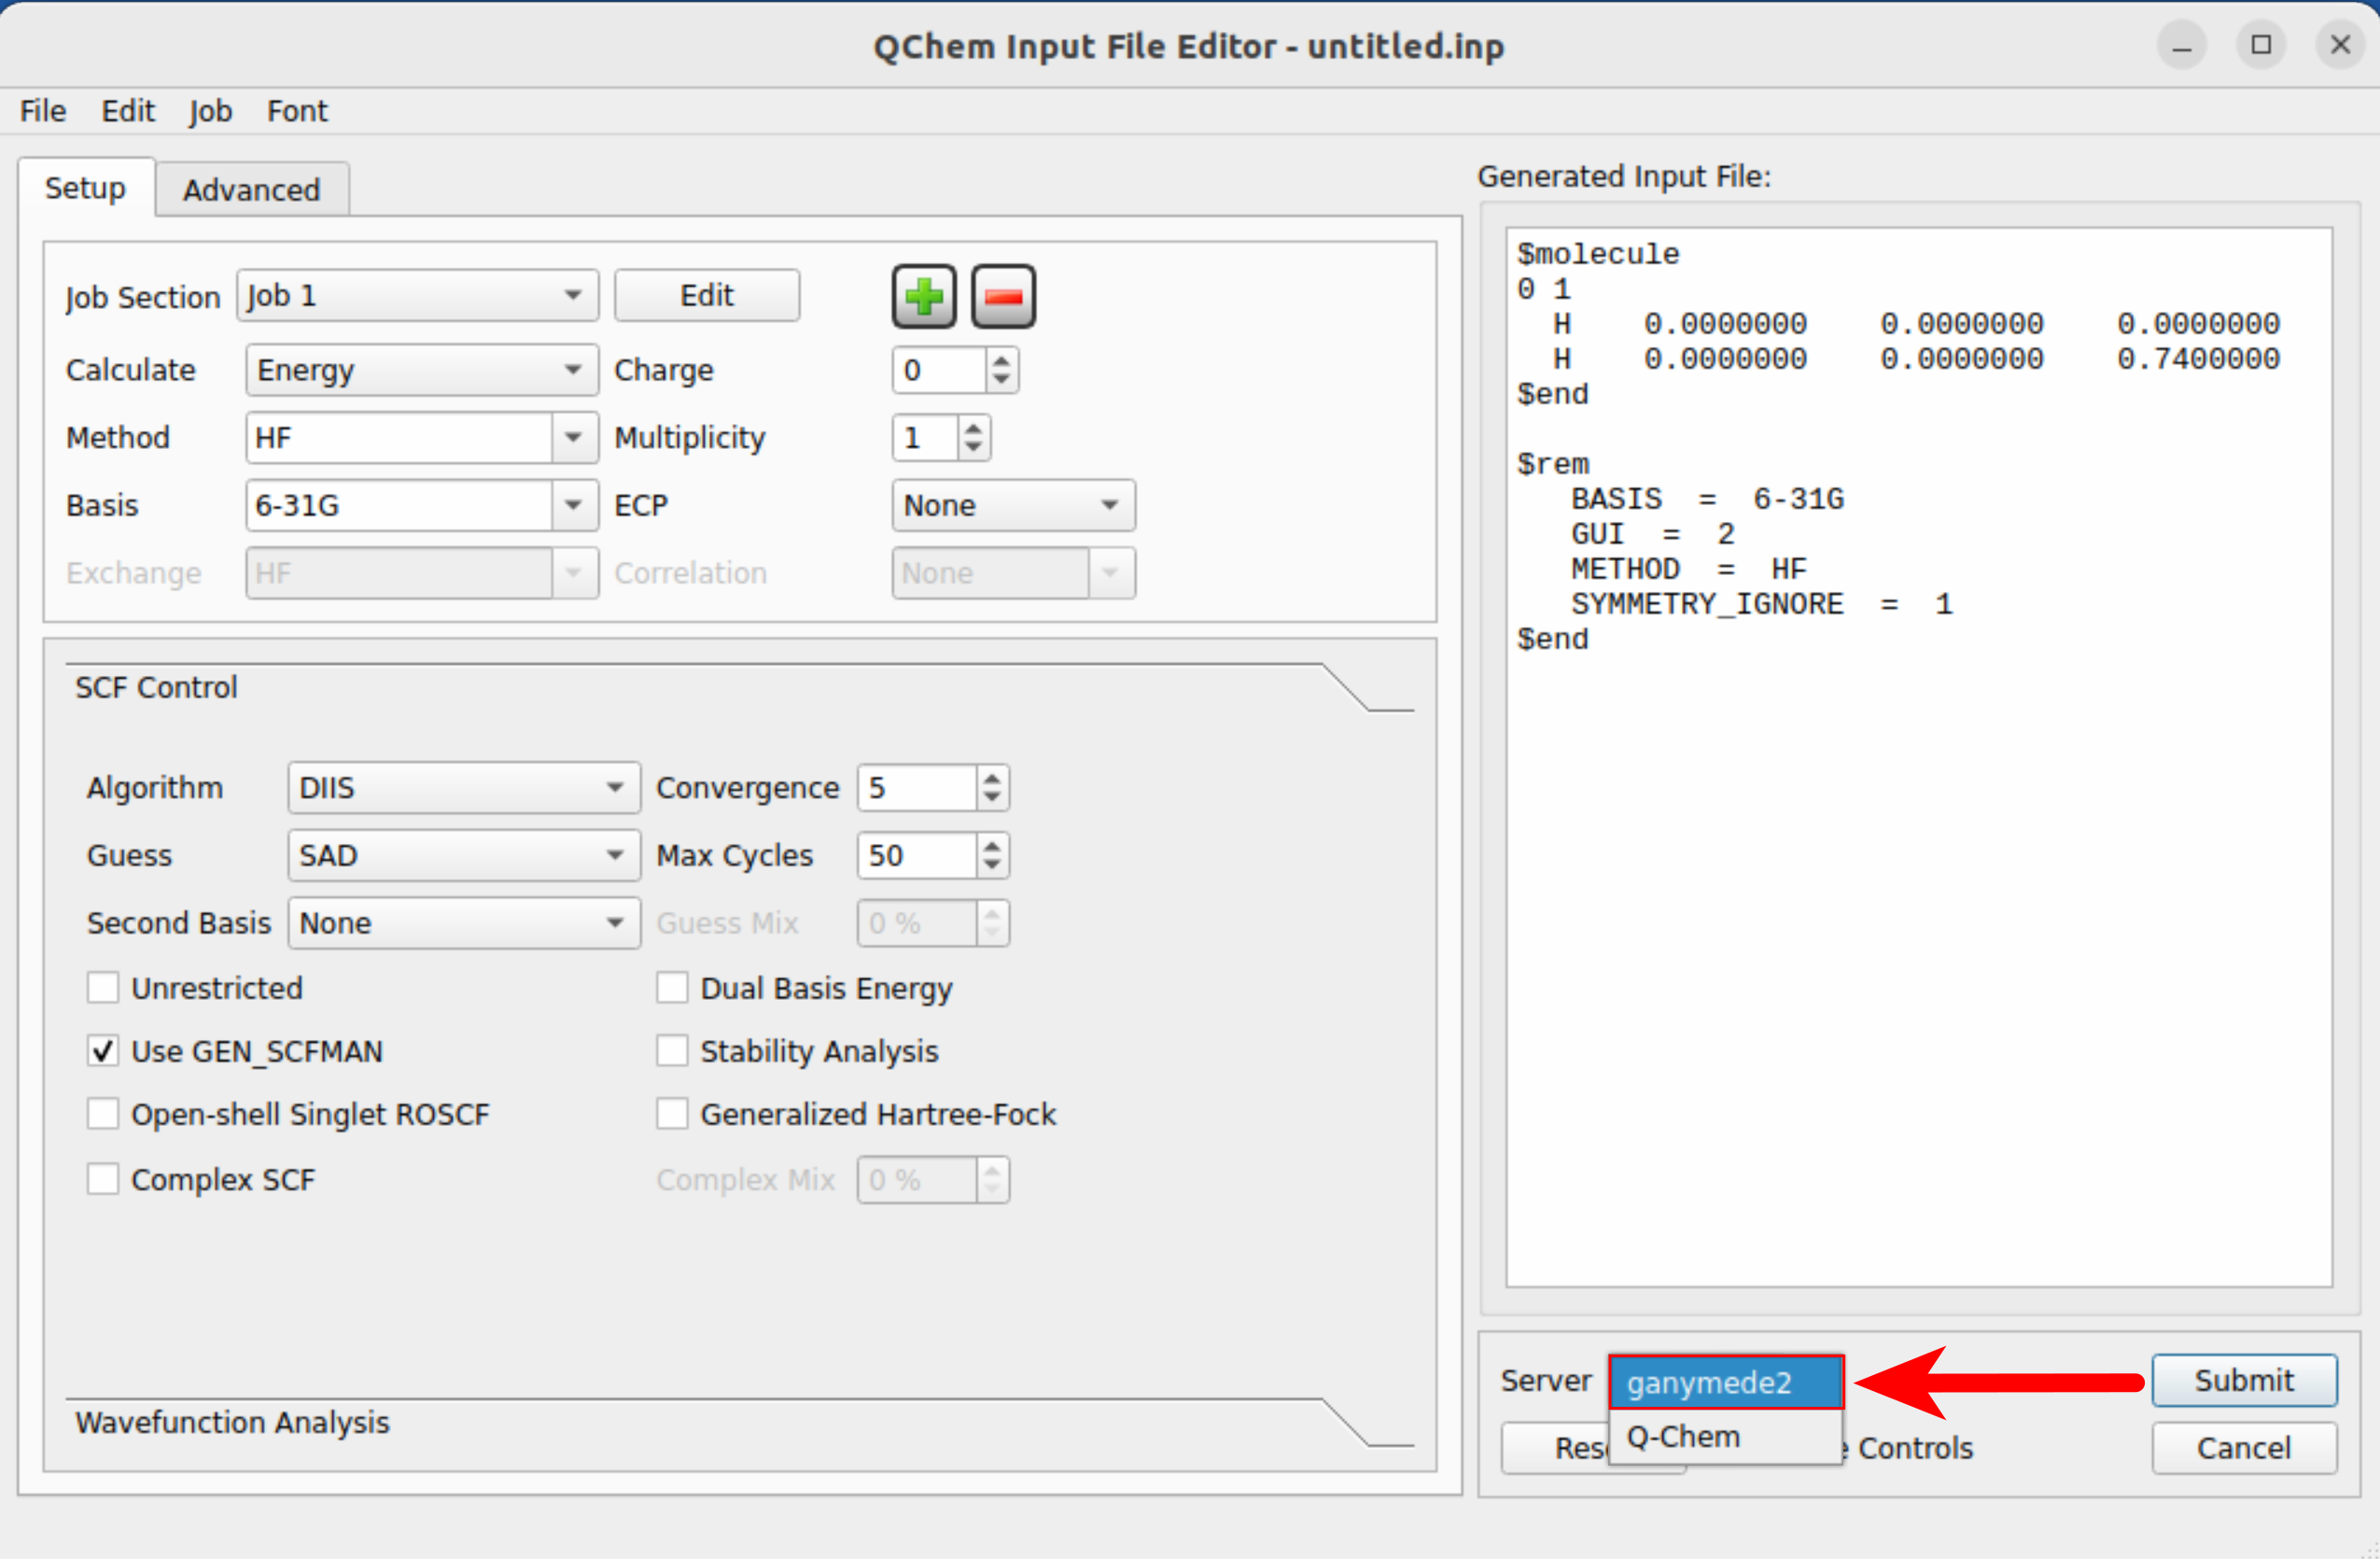
\includegraphics[width=0.8\textwidth]{iqmol_submit_job.png}
        \caption{Submitting a Job in IQmol}
        \label{fig:iqmol_submit_job}
    \end{figure}

    \item The following steps have to be done every time you start IQmol:
    \begin{enumerate}
        \item Upon submission, a prompt may appear to add the Host to known hosts file. Click \textbf{Yes}.
        \item If using password authentication, enter your \textbf{NetID password} when prompted.
    \end{enumerate}

    \item Choose a \textbf{Folder Name} for your job files. \textbf{Note: Do not use spaces in the folder name.}

    \item Configure the job settings:
    \begin{itemize}
        \item \textbf{Queue}:
        \begin{itemize}
            \item If you are enrolled, select the \texttt{6v39} partition.
            % \item If you are auditing, choose \texttt{normal}.
        \end{itemize}
        \item \textbf{Wall Time}: Set the maximum time for your job. Ensure that you allocate enough time, but do not exceed 48 hours.
        \item \textbf{CPUs}: Select the number of CPUs you wish to use. Do not exceed 8 CPUs per job.
    \end{itemize}

    \begin{figure}[H]
        \centering
        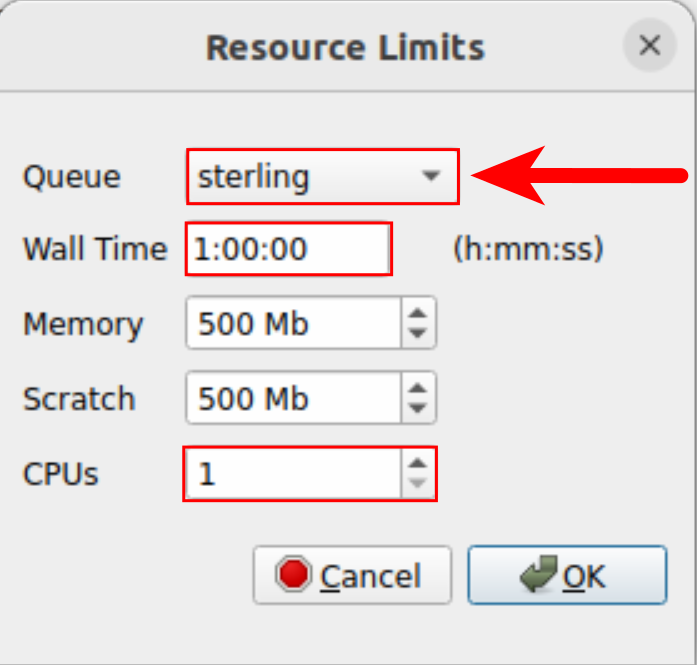
\includegraphics[width=0.7\textwidth]{iqmol_job_resources.png}
        \caption{Configuring Job Resources}
        \label{fig:iqmol_job_resources}
    \end{figure}

    \item Click \textbf{OK} to submit the job.
\end{enumerate}

\section{Conclusion}

You have successfully configured IQmol to connect to the server and submitted a job.
Remember to monitor your jobs on the server. If you encounter any issues, contact your system administrator for assistance.

\end{document}

